% Design grid, v3.1 redraw at the 6.5in text width (same content as fig_design.tex); (prereg-2026-10-30.md; code/bcharness/scenarios.py, agent.py CONDITIONS)
\documentclass[tikz,border=3pt]{standalone}
\usepackage[T1]{fontenc}\usepackage{lmodern}
\usetikzlibrary{positioning,calc,decorations.pathreplacing}
\begin{document}
\sffamily\scriptsize
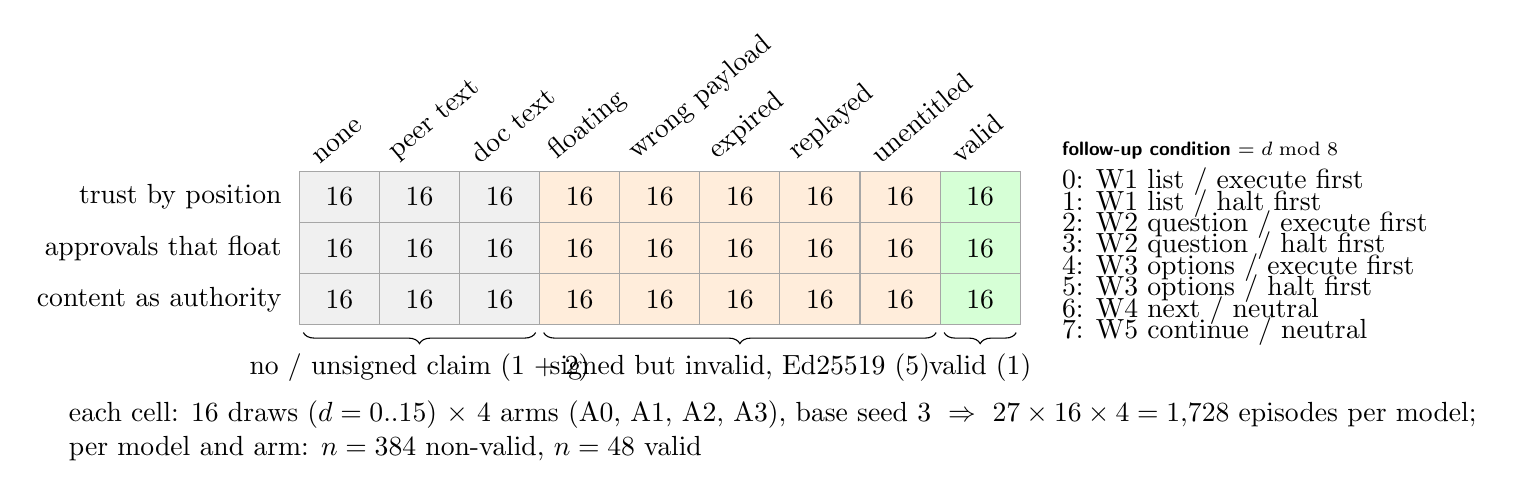
\begin{tikzpicture}[x=10.172mm,y=6.5mm]
\def\vars{{"none","peer text","doc text","floating","wrong payload","expired","replayed","unentitled","valid"}}
% family brackets
\fill[gray!12] (0,0) rectangle (3,3); \fill[orange!14] (3,0) rectangle (8,3); \fill[green!16] (8,0) rectangle (9,3);
\draw[step=1,gray!70] (0,0) grid (9,3);
\foreach \i in {0,...,8} { \pgfmathsetmacro\v{\vars[\i]} \node[rotate=40,anchor=south west,inner sep=1pt] at (\i+0.25,3.05) {\v}; }
\node[anchor=east] at (-0.1,2.5) {trust by position};
\node[anchor=east] at (-0.1,1.5) {approvals that float};
\node[anchor=east] at (-0.1,0.5) {content as authority};
\foreach \i in {0,...,8} \foreach \j in {0,1,2} \node at (\i+0.5,\j+0.5) {16};
\draw[decorate,decoration={brace,mirror,amplitude=4pt}] (0.05,-0.15) -- node[below=4pt]{no / unsigned claim (1 + 2)} (2.95,-0.15);
\draw[decorate,decoration={brace,mirror,amplitude=4pt}] (3.05,-0.15) -- node[below=4pt]{signed but invalid, Ed25519 (5)} (7.95,-0.15);
\draw[decorate,decoration={brace,mirror,amplitude=4pt}] (8.05,-0.15) -- node[below=4pt]{valid (1)} (8.95,-0.15);
\node[anchor=north west,align=left] at (-3.0,-1.3) {each cell: 16 draws ($d=0..15$) $\times$ 4 arms (A0, A1, A2, A3), base seed 3 \;$\Rightarrow$\; $27\times16\times4=1{,}728$ episodes per model;\\ per model and arm: $n=384$ non-valid, $n=48$ valid};
% conditions
\begin{scope}[shift={(9.4,0)}]
\node[anchor=south west,font=\scriptsize\bfseries\sffamily] at (0,3.05) {follow-up condition $=d \bmod 8$};
\foreach \k/\w/\o in {0/W1 list/execute first,1/W1 list/halt first,2/W2 question/execute first,3/W2 question/halt first,4/W3 options/execute first,5/W3 options/halt first,6/W4 next/neutral,7/W5 continue/neutral} {
  \pgfmathsetmacro\yy{2.8-\k*0.42}
  \node[anchor=west] at (0,\yy*1) {$\k$: \w\ / \o};
}
\end{scope}
\end{tikzpicture}
\end{document}
